\documentclass[12pt]{article}
\usepackage[paper=a4paper,left=1.5cm, right=1.5cm, top=1.5cm]{geometry}
\usepackage[utf8]{inputenc}
\usepackage{graphicx}
\setlength{\parindent}{4em}
\setlength{\parskip}{1em}
\usepackage{graphicx}

\title{\textbf{Nanoparticles : Medical Imaging Advancement}}
\author{Sajal Harmukh \\ Roll No - 18111046 \\ \textit{Department of Biomedical Engineering} \\ National Institute of Technology, Raipur }
\date{01\textsuperscript{st} April 2022}

\begin{document}

\maketitle

\section*{Abstract}

To study and summarise the recent advancement and the emerging research on the use of nanoparticles in the biomedical imaging and to lookout for an early detection and diagnosis of the disease, which is the driving force in the field of medical imaging.

\section*{Introduction}
Nanomaterials, such as nanoparticles, nanorods, nanosphere, nanoshells, and nanostars, are very commonly used in biomedical imaging. They make excellent drug carriers, imaging contrast agents, photothermal agents, photoacoustic agents, and radiation dose enhancers, among other applications. Recent advances in nanotechnology have led to the use of nanomaterials in many areas of functional imaging, cancer therapy. Nanotechnology has arisen as a multidisciplinary research endeavour focused at understanding and controlling materials through the convergence of concepts from engineering, chemistry, biology, medicine, and other disciplines [1]. Recent technical advancements in the creation of various types of nanoparticles clearly demonstrate the significance of nanoparticles in biological imaging applications [2,3]. Nanoparticles have diameters ranging from 1 to 100 nm, according to the National Nanotechnology Initiative (NNI). Because of their size similarities to significant naturally occurring nanoparticles such as viruses, somewhat bigger particles are frequently defined as nanoparticles within the biomedical community as well. At these sizes, nanoparticles exhibit unique features that distinguish them from molecules and bulk materials.\\ Nanoparticles have been discovered to target tumours passively through the increased permeability and retention effect (EPR) [4], or particular organs such as the lymphatic system by molecular sieving [5], without the need of exogenous targeting ligands. At these sizes, nanoparticles exhibit unique features that distinguish them from molecules and bulk materials. Nanoparticles have been discovered to target tumours passively through the increased permeability and retention effect (EPR) [4], or particular organs such as the lymphatic system by molecular sieving [5], without the need of exogenous targeting ligands. The creation of molecular probes for the viewing of cellular function, characterisation, and measurement of molecular processes in live creatures at the cellular and molecular level without perturbing them is referred to as molecular imaging [7]. There have been developments in nanomaterials during the last ten years, such as the invention of hundreds of nanoparticles (NPs)-based probes for molecular imaging.
The use of nanoparticles (NPs) has improved nearly all main imaging techniques, including magnetic resonance imaging (MRI), positron emission tomography (PET), and optical imaging. 

\begin{figure}[htp]
    \centering
    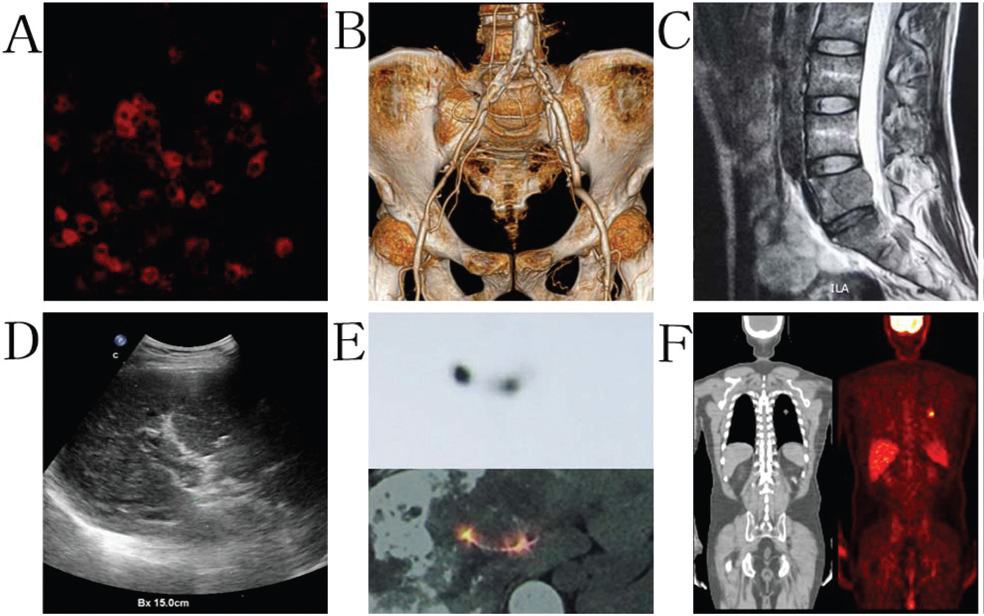
\includegraphics[width=10cm]{6.png}
    \caption{\textit{A is a fluorescence picture of tumour cells; B is a CT image of arterial stenosis; C is an MRI image of lumbar vertebral metastases; D is a US detection of portal vein thrombosis; E is a SPECT assessment for 125I seed implantation; and F is a PET detection of lung cancer. All photos were collected from China Medical University's medical imaging research institute.}}
    \label{fig:1}
\end{figure}
Almost all major imaging methods, including magnetic resonance imaging (MRI), positron emission tomography (PET), and optical imaging, have been enhanced by the introduction of nanoparticles (NPs). SPECT (computed tomography) with fluorescence imaging (Fig. 1). To increase lesion identification, multiple imaging modalities are frequently combined. 

\section*{Nanoparticles in imaging }

At the moment, a wide range of nanoparticle systems are being investigated for their possibility in cellular imaging, with several applications aimed at cancer diagnosis or treatment [9]. Particle charge, size, shape, and hydrophilicity continue to be among the most important properties of nanoparticles for effective delivery to the target. Polyethylene glycol (PEG) particles have been explored broadly as a successful means to give hydrophilic 'secrecy' properties, ordinarily yielding diminished vague adsorption of serum proteins in vivo, in this manner creating longer flow times [10]. Different sorts of nanoparticle are currently being scrutinized, including strong lipid nanoparticles, liposomes, micelles, nanotubes, metallic nanoparticles, quantum spots, dendrimers, polymeric nanoparticles and iodinated nanoparticles. Metallic nanoparticles have massive potential as X-beam contrast imaging specialists attributable to their powerful X-beam ingestion and low harmfulness profiles saw over brief spans in creatures [12,13]. Gold nanoparticles stand out enough to be noticed inferable from the expected biocompatibility, somewhat low transient harmfulness, and high ingestion coefficient and actual thickness contrasted and iodine (gold 79(Z), 5.16 cm/g, 19.32 g/cm ; iodine 53(Z), 1.94 cm/g, 4.9 g/cm ). Consequently, there is a critical interest for the amalgamation of these kinds of nanoparticle under harmless circumstances that decrease concerns with respect to the poisonousness possibly prompted by the lessening specialists and response conditions. Targeting nanoparticles could be a significant improvement over current contrast media. The addition of targeting ligands allows for increased specificity and nanoparticle–tumour interactions in diseased tissues [16,17]. Numerous functionalized nanoparticles have been intended to have a high liking for different destructive cell surface receptor proteins that are overexpressed on a wide scope of disease cells (Figure 2A) .\\
\begin{figure}[htp]
    \centering
    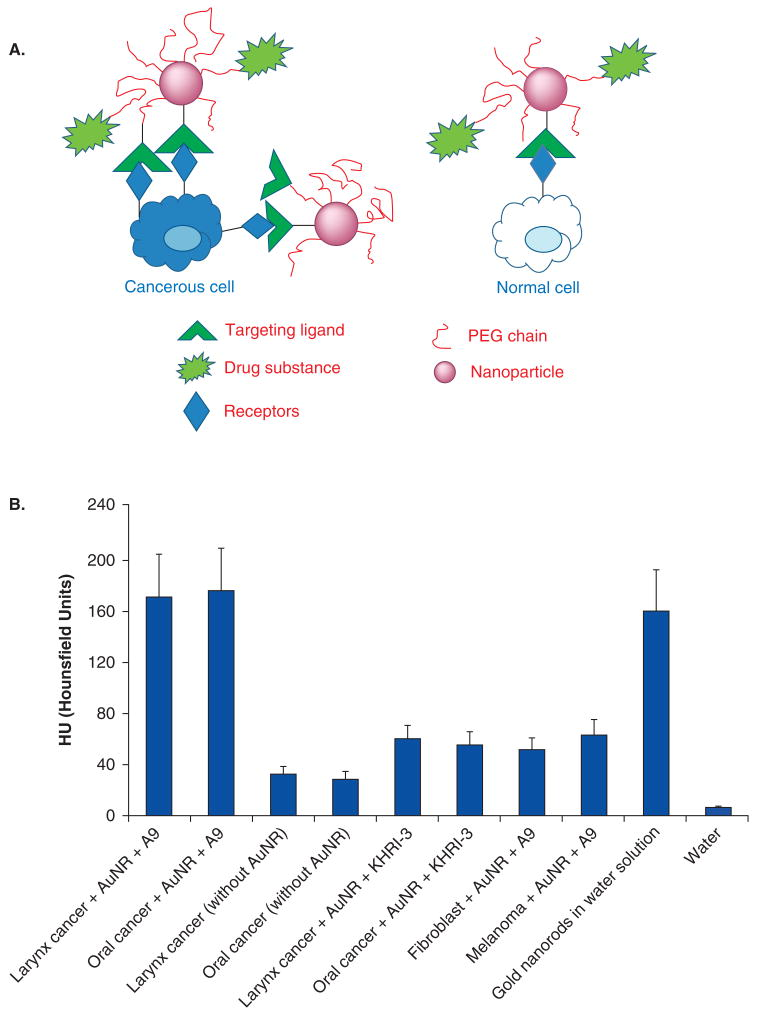
\includegraphics[width=10cm]{1.jpg}
    \caption{\textit{A. Nanoparticle targeting cancerous cell ,  B. CT attenuation (HU) of A9-antibody-coated gold nanorods (AuNR) in the presence of cancerous and non-cancerous cells}}
    \label{Fig:2}
\end{figure}
\\
The multivalent show of little particles may for sure be because of intervening somewhat solid associations between functionalized nanoparticles and the expected cells and biomolecules [18]. The utilization of little particles as an option in contrast to antibodies permits further enhancement of the limiting proclivity and explicitness by changing the thickness of focusing on atoms [18]. Clinical imaging has worked on altogether in late many years and permits us to acquire definitively physical data by means of different modalities. Nanoparticles have a huge influence in clinical imaging as examined underneath :

\section*{Applications of nanoparticles in imaging }
\subsection*{Gold Nanoparticle} 
Because of their unique chemical, physical, and optical properties, inorganic nanoparticles are emerging as versatile imaging tools [20]. Gold nanoparticles were discovered more than a century ago, and due to their surface chemistry, projected biocompatibility, low short-term toxicity, high atomic number, and high X-ray absorption coefficient, gold nanoparticles have recently received significant interest for use in a variety of imaging technologies. There are reliable and simple methods for creating gold nanoparticles with precise control over particle size and shape [21,22]. Gold nanoparticles can be synthesised under relatively benign conditions, which is significant given the growing concerns about nanomaterial safety and toxicity in biomedical applications [21,23].
 Spherical gold nanoparticles with diameters ranging from a few to several hundred nanometers may be easily produced with great precision and accuracy in aqueous or organic solvents. As a rule, decrease of gold salts (e.g., AuCl) prompts the nucleation of gold particles [25,26]. As gold nanoparticles are not steady, a settling specialist is required that is genuinely adsorbed or artificially bound to the gold surface. The age of gold nanoparticles in fluid medium regularly utilizes either trisodium citrate or sodium borohydride as decreasing specialists [27,28]. Definitively controlling citrate fixation brings about the development of little and uniform gold nanoparticles
\begin{itemize}
    \item \textbf{ Gold nanoparticle in Computed tomography} - gold nanoparticles have unique x-ray attenuation characteristics and are easily modified on the surface. To make an effective contrast agent, Au NPs can be functionalized with glucosamine [39]. Gold nanoparticles have a high x-ray absorption coefficient and can be used to assess tumours with improved permeability and retention effects utilising CT (EPR). Au NPs were coupled with PEG chains and tumour biomarkers in a breast cancer investigation (human epidermal growth factor 2). Because of their precise aiming capabilities, they were able to produce an improved image in CT [40]. A mesenchymal immature microorganism is a
sort of grown-up foundational microorganism that has high potential in cell based regenerative treatment and can treat different ailments, for example, immune system, neurodegenerative, and cardiovascular infection. Their most unusual trait is the ability to move into other tissues, and tracking this migration is extremely useful for researching metastases. Gold nanoparticles (1.9 nm) were used as an X-ray CT contrast agent to identify malignancies in mice by Hainfeld et al. [13].
The injected gold nanoparticles were not identified in the blood after 24 hours, but they accumulated significantly in the kidney (10.62 percent injected dose/g [ID/g]), tumour (4.2 percent ID/g), liver (3.6 percent ID/g), and muscle (1.2 percent ID/g) after just 15 minutes. Kattumuri et al. recently shown the effective usage of gum Arabic stabilised gold nanoparticles as a possible biocompatible X-ray CT contrast agent [34]. The nanoparticles' limited binding to blood plasma showed that they were stable in vivo. PEG-coated nanoparticles administered intravenously into rats demonstrated much longer blood circulation duration (> 4 h) than the routinely used iodine contrast agent iopromide (10 min) [35]. Until recently, CT was not regarded a molecular imaging modality in the same way that magnetic resonance imaging (MRI) and other nuclear medicine imaging modalities (single-photon-emission computed tomography [SPECT], positronemission tomography [PET], and so on) were.
Popovtzer et al., on the other hand, showed the use of gold nanoparticles as target-specific agents in vitro using a typical clinical CT [16]. It is vital to remember that the quantity of gold content per unit volume is important in CT imaging, regardless of particle shape and size. The enhanced X-ray attenuation in targeted SCC [Squamous cell carcinoma] cells as compared to normal cells validates the fundamental premise for the creation of molecular X-ray CT imaging agents (Figure 2B).

\end{itemize}

\subsection*{Quantum Dots}
Quantum dots (QDs) are fluorescent semiconductor nanocrystals (sizes ranging from 1 to 100 nm) with distinct optical and electrical characteristic. QDs have near-unity quantum yields and substantially higher brightness than most dyes (10 – 100 times) when compared to organic dyes and fluorescent proteins. Quantum dots also have a broad absorption spectrum, a narrow linewidth in emission spectra, continuous and tunable emission maxima due to quantum size effects, a relatively long fluorescence lifetime (5 to > 100 ns compared to 1 – 5 ns in organic dyes), and negligible photobleaching (100 – 1000 times less than fluorescent dyes) over minutes to hours. These properties make QDs invaluable for clinical imaging applications when matched with the potential for in vivo focusing of explicit cells (e.g., marking neoplastic cells, DNA, and cell layer receptors) later formation with explicit bioactive moieties. One downside is the squinting peculiarity seen in these semiconductors. Engineered procedures exist for the exact control of QD size and piece, which in enormous part control the retention and outflow attributes. The benefits of QDs over other biological labelling techniques (e.g., fluorescent dyes and radioisotopes) are expected to increase their adoption. Quantum dots, like all other nanoparticles, have a significant number of atoms on their surface that are occupied by unoccupied atomic or molecular orbitals. Quantum dots feature a metalloid crystalline core (e.g., CdSe) and a shell (e.g., ZnS) that protects the core.
\begin{figure}[htp]
    \centering
    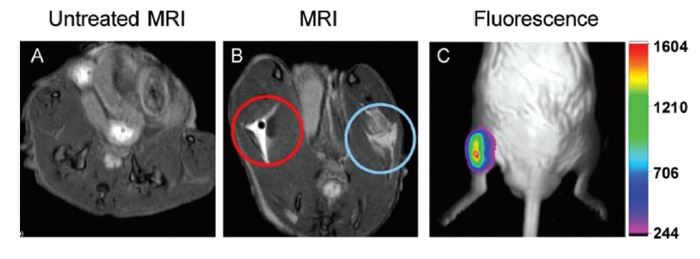
\includegraphics[width=10cm]{4.jpg}
    \caption{\textit{T1 MRI contrast in a compact plasmonic nanoparticle
with enhanced fluorescence synthesized by a multilayer core–shell
nanostructure, known as nanomatryoshka (NM).}}
    \label{Fig:2}
\end{figure}
\begin{itemize}
\item \textbf{QD in medical imaging } - Fluorescence imaging allows for the viewing of cellular features in real time. Long-term imaging, however, is difficult due to the weak light stability of organic fluorescent dyes. Graphene quantum dots are a viable option. Fluorescence imaging offers significant benefits over other imaging modalities since it has high sensitivity and is non-invasive. However, because it is an optical approach, it has limited tissue penetration depth. Akerman et al. found that CdSe/Zns QDs coated with PEG and a lung-targeting peptide accumulated significantly in the lungs of mice [66].
Gao et al. recently disclosed the invention of multifunctional QD-based nanoparticle probes for in vivo imaging of human prostate cancer in mice. The shell material in conventional QDs (type I) is constructed of a high band gap material with a higher energy conduction band than the core and a lower valence band than the core. Type II QDs, on the other hand, are made of core–shell materials with offset band gaps. Multiple components, such as gadolinium and manganese, can be carefully included into QDs to create multimodal imaging agents [73]. In this vein, Jin et al. created hybrid QDs by carefully integrating Gd into QDs to provide dual mode (fluorescence/magnetic resonance) imaging. Similarly, Yong devised a novel method for manufacturing manganese-doped QDs as multimodal targeted probes for pancreatic cancer imaging.
\end{itemize}


\subsection*{Iron oxide Nanoparticles}
Magnetic nanoparticles have gotten a lot of interest because of their potential use in optical, magnetic, and electrical devices. Metal nanoparticles of iron oxide, like gold nanoparticles and QDs, are predicted to have good biocompatibility at low concentrations, high magnetic saturation, and functional surfaces. Magnetic iron oxide nanoparticles have been functionalized with antibodies, nucleosides, proteins, and enzymes to target sick tissues like tumours [77,78]. Super para-magnetism and high field irreversibility are seen in iron oxide nanoparticles, which are caused in part by the size and surface features of individual nanoparticles. Magnetic nanoparticles are chemically and structurally comparable to gold nanoparticles and QDs. The core material is often highly superparamagnetic iron oxide, and biocompatible polymers such as dextran may be employed as a coating material [83]. SPION (superparamagnetic iron oxide nanoparticles) contain high magnetic moments and are ideal for use as T2 contrast agents in MRI.
For the reasons stated earlier, there has been a great deal of interest in producing iron oxide nanoparticles with regulated shapes and sizes. To answer this problem, numerous synthetic methodologies, including microemulsion [89], sol-gel [90], sonochemical synthesis [91], and co-precipitation procedures [92,93], have been developed. The most prevalent process appears to be aqueous co-precipitation of nanoparticles in the presence of a coating substance. Hydrophobic ligands and organic solvents are used in methods that claim exquisite control over particle size and shape. Water insoluble nanoparticles may be produced using a multifunctional ligand system (e.g., 2,3-dimercapitosuccinic acid [DMSA]) that allows the transfer of nanocrystals to an aqueous phase to increase biocompatibility. Doping iron oxide nanoparticles with other metals may boost their magnetic characteristics even more. Nanoparticles are often doped to generate MFe O (M = Mn, Fe, Co, or Ni), in which the Fe in Fe O is replaced by metal 'M' [97].
\begin{itemize}
    \item \textbf{Iron oxide as nanoparticle in MRI } - MRI is a non-invasive medical
    imaging method that is extensively used in clinical medicine to evaluate tissue structure and function [7,82,104], and it typically gives more contrast between soft tissues than computer tomography (X-ray CT). The behaviour, alignment, and interaction of protons in the presence of a magnetic field provides the basis for MRI. Protons in the tissue are disrupted from B inside a high magnetic field; contrast compounds are employed to modify longitudinal (T1) or transverse (T2) relaxation durations, which may be monitored by MRI. MRI eliminates the need for radiation and can provide greater spatial resolution. One notable advantage of iron oxide nanoparticles is their biocompatibility and ease of detection at low doses. MRI contrast agents based on erric oxide have the ability of lowering T2 relaxation time to dark pictures on T2 weighted imaging, resulting in 'negative' MRI contrast. In biomedical imaging applications, three kinds of iron-based nanoparticles are being employed. The first category is SPIO, which has received the most attention in terms of study. The size of SPIO nanoparticles goes from a few to thousands of nanometers. In light of their general breadth (hydrodynamic measurement), they are arranged into enormous SPIO (LSPIO) nanoparticles at 300-35,000 nm; standard SPIO (SSPIO) nanoparticles at 60-150 nm; minuscule SPIO (USPIO) nanoparticles at 10-40 nm; and monocrystalline iron oxide nanoparticles at 10-30 nm, which is a subset of USPIO. SPIONs have a high saturation magnetization and magnetization loss in the absence of a magnetic field, and these nanoparticles are thought to be less hazardous than optical imaging agents. MRI has been extensively utilised to analyse cell movement (cellular trafficking) using magnetic nanoparticle probes [113,114]. Xie et al. created c(RGDyK)-conjugated ultra-small iron oxide nanoparticles (USPION) for targeting integrin-rich tumour cells. USPIONs have been employed in malignancies to overcome nonspecific uptake, clearance, and extravasation [115]. Engineered nanoparticles with high and controllable magnetism outperform standard iron oxide contrast agents in terms of sensitivity and dosage. MRI contrast agents containing ferric oxide have been employed in a variety of biomedical imaging applications, including molecular imaging, gene monitoring, cell tracking, blood pool imaging, lymph node identification, and cancer diagnosis.

\end{itemize}

\subsection*{Carbon Nanotubes} 
Carbon nanotubes (CNTs) have captivated scientists since their discovery in the soot of an arc discharge device by Iijima in 1991 [117]. Their unusual optical, electrical, and mechanical capabilities have piqued their interest. CNTs are similar to rolled-up monolayered graphite sheets. Structures with single and multiple walls can be built. CNTs' extraordinary properties, including as high electrical and thermal conductivity and high tensile strength, suggest that they might be used as field emission devices, tips for scanning microscopy, nanoscale transistors, or components for composite materials. The NIR fluorescence characteristics of single-walled carbon nanotubes (SWNT) and surface functionalization are now hot topics in biological imaging. NIR fluorescence occurs in the physiologically transparent area (700–1300 nm), when autofluorescence, absorption, and scattering by blood and tissue are minimal. SWNTs are intriguing as imaging contrast agents [119,120] and biological sensors [121] due to their unique NIR fluorescence characteristics [118]. Surface functionalized multi-walled carbon nanotubes (MWNTs) have also been effectively employed in bioimaging [122]. Carbon nanotubes with diameters in the nm range and lengths in the m range may be commercially produced as single-walled or multiwalled structures.\\
For CNT manufacture, several techniques have been devised, including arc discharge and evaporation, laser ablation [123], and chemical vapour deposition (CVD) [124]. Although the laser ablation approach is not currently scaleable, it is capable of producing SWNTs with a purity of up to 90 $\%$. Arc discharge evaporation is likely the simplest and most used method for producing CNTs. CNTs are made by arc evaporating two carbon rods (10 or 20 mm in diameter) arranged end to end with a 1 mm gap in an inert gas atmosphere at 50–700 mbar. Direct current evaporates the two carbon rods.  The anode evaporates, leaving rod-shaped tubes on the cathode.

\begin{itemize}
    \item \textbf{CNTs in biomedical imaging } -Carbon nanotubes are projected to have a wide range of uses in biomedicine, including imaging and treatment, due to their ease of internalisation by live cells. The main disadvantages of CNTs are their insolubility in many types of solvents and the possibility that CNTs may be toxic to organisms. However, it has been demonstrated that surface functionalized carbon nanotubes (f-CNTs) are extremely soluble in water. CNT-based bioimaging applications for cancer cell annihilation, detection, and dynamic imaging have been established. Confocal microscopy was used to examine SWNTs covalently coupled to visible-wavelength fluorophores in cells [119,120]. \\The ability of the f- CNTs to pass the cell membrane was proven by clear pictures from epifluorescence and confocal imaging. To investigate the cytotoxicity of SWNT intake, researchers used a spectrofluorometer and a fluorescence microscope adapted for NIR imaging [128]. The detection and imaging of SWNT fluorescence provides a strong tool for tracing SWNT interactions with tissues, cells, and organisms.
\end{itemize}

\subsection*{Dendrimers}
Dendrimers are well-defined, highly branched molecules with excellent structural control and low polydispersity [129-132]. Dendrimers are interesting particulate systems for biological applications due to their tunable size variation, availability of a large number of reactive sites, and inner void space [129]. Dendrimers are orchestrated in a stepwise design utilizing either the 'different' or 'joined' approach. Tamalia's disparate strategy begins with a multifunctional center and afterward adds monomers more than once to dramatically develop sub-atomic mass and surface ends. These functional groups, which can have anionic, neutral, or cationic terminals, can be employed to change the overall structure as well as the chemical and physical characteristics. Therapeutic compounds can be encapsulated or linked to the surface groups of dendrimers, making them extremely bioavailable and biodegradable.
Magnevist, a gadolinium(III)-diethylenetriaminepentaacetic acid (Gd-DTPA) complex, is a popular MRI contrast agent, although its quick elimination and non-specificity limit its value. Dendrimer contrast agents with molecular weights of 8508 and 139,000 Da, for example, had half-lives of 40 10 and 200 100 min, respectively, compared to 24 4 min for Gd-DTPA [137,138]. Dendrimers offer a lot of potential in nanomedical imaging and MRI. Their stiffness, low polydispersity, and simplicity of surface modification are all highly novel features.
Dendrimers are used in MRI for cell tracking, lymph node imaging, blood pool imaging, and tumor-targeted theranostic. Gadolinium is a paramagnetic agent having one of the greatest diamagnetic properties relaxivities caused by the big dendrimer molecules' high rotational correlation time, as stated at the start.

\section*{Conclusion}
Recent breakthroughs in nanotechnology have resulted in significant advancements in synthetic processes that profit from the creation of numerous nanomaterials, such as nanoparticles, nanocages, nanodiamonds, and so on. These nanoparticles can function as highly effective contrast agents in a variety of medical imaging modalities and provide a wide range of alternatives in current cancer therapy. The use of nanoparticles in biological imaging in the future seems promising. Nontoxic, biocompatible, and biodegradable nanoparticles that resist nonspecific organ absorption and RES should be developed further in synthesis procedures. Finally, developing concepts that use nanoparticles with various functionalities (e.g., imaging and therapeutic) should carefully examine the regulatory complexities of these sorts of combination approaches.
Future initiatives include further refining diverse nanomaterials and unravelling the precise processes between the cell and nanoparticles in order to produce better imaging and therapeutic effects, as well as accelerating the translation of nanomaterials into clinical practise.

\section*{References}
[1]. Niemeyer CM. Nanoparticles, proteins, and nucleic acids: biotechnology meets materials science. Angew Chem Int Ed. 2001;40(22):4128–58. \url{[PubMed] [Google Scholar]}
\section*{}
[2]. Ferrari M. Cancer nanotechnology: opportunities and challenges. Nat Rev Cancer. 2005;5(3):161–71. \\[3]. Forrest ML, Kwon GS. Clinical developments in drug delivery nanotechnology. Adv Drug Deliv Rev. 2008;60(8):861–2. \\
[4]. Greish K. Enhanced permeability and retention of macromolecular drugs in solid tumors: A royal gate for targeted anticancer nanomedicines. J Drug Target. 2007;15(7-8):457–64. \\
[5]. Hawley AE, Illum L, Davis SS. Preparation of biodegradable, surface engineered PLGA nanospheres with enhanced lymphatic drainage and lymph node uptake. Pharm Res. 1997;14(5):657–61. \\
[6]. Davis ME, Chen Z, Shin DM. Nanoparticle therapeutics: an emerging treatment modality for cancer. Nat Rev Drug Discov. 2008;7(9):771–82. 



 \end{document}
